\title{COM S 352 Homework 8}
\author{Alec Meyer}

\date{\today}

\documentclass[11pt]{article}
\usepackage{changepage}
\usepackage{graphicx}
\usepackage{amsmath}
\graphicspath{ {./images/} }
\newcommand\tab[1][1cm]{\hspace*{#1}}
\usepackage{amssymb}


\begin{document}
\maketitle

\section*{Question 1}
\begin{itemize}
    \item \textbf{a.}
        Yes, the state will change from running to blocked.
    \item \textbf{b.}
        No, because an address reference is resolved in the page table.
        The state will stay running.
\end{itemize}
\section*{Question 2}
\begin{itemize}
    \item \textbf{a.}
        Offset: 0xDD\\
        Page num: 0x2\\
        Page 2 = Frame 10 = 0xA\\
        Physical adress: 0xADD
    \item \textbf{b.}
        Offset: 0xE6\\
        Page num: 0x4\\
        page 4 = page fault\\
        set to 9\\
        Physical address: 0x9E6
    \item \textbf{c.}
        Offset: 0x4A\\
        Page num: 0x9\\
        page 9 = frame 1 = 0x1\\
        Physical address: 0x14A
    \item \textbf{d.}
        Offset: 0x16\\
        Page num: 0x3\\
        Page 3 = page fault = 15 = 0xF\\
        Physical address: 0xF16
\end{itemize}
\section*{Question 3}
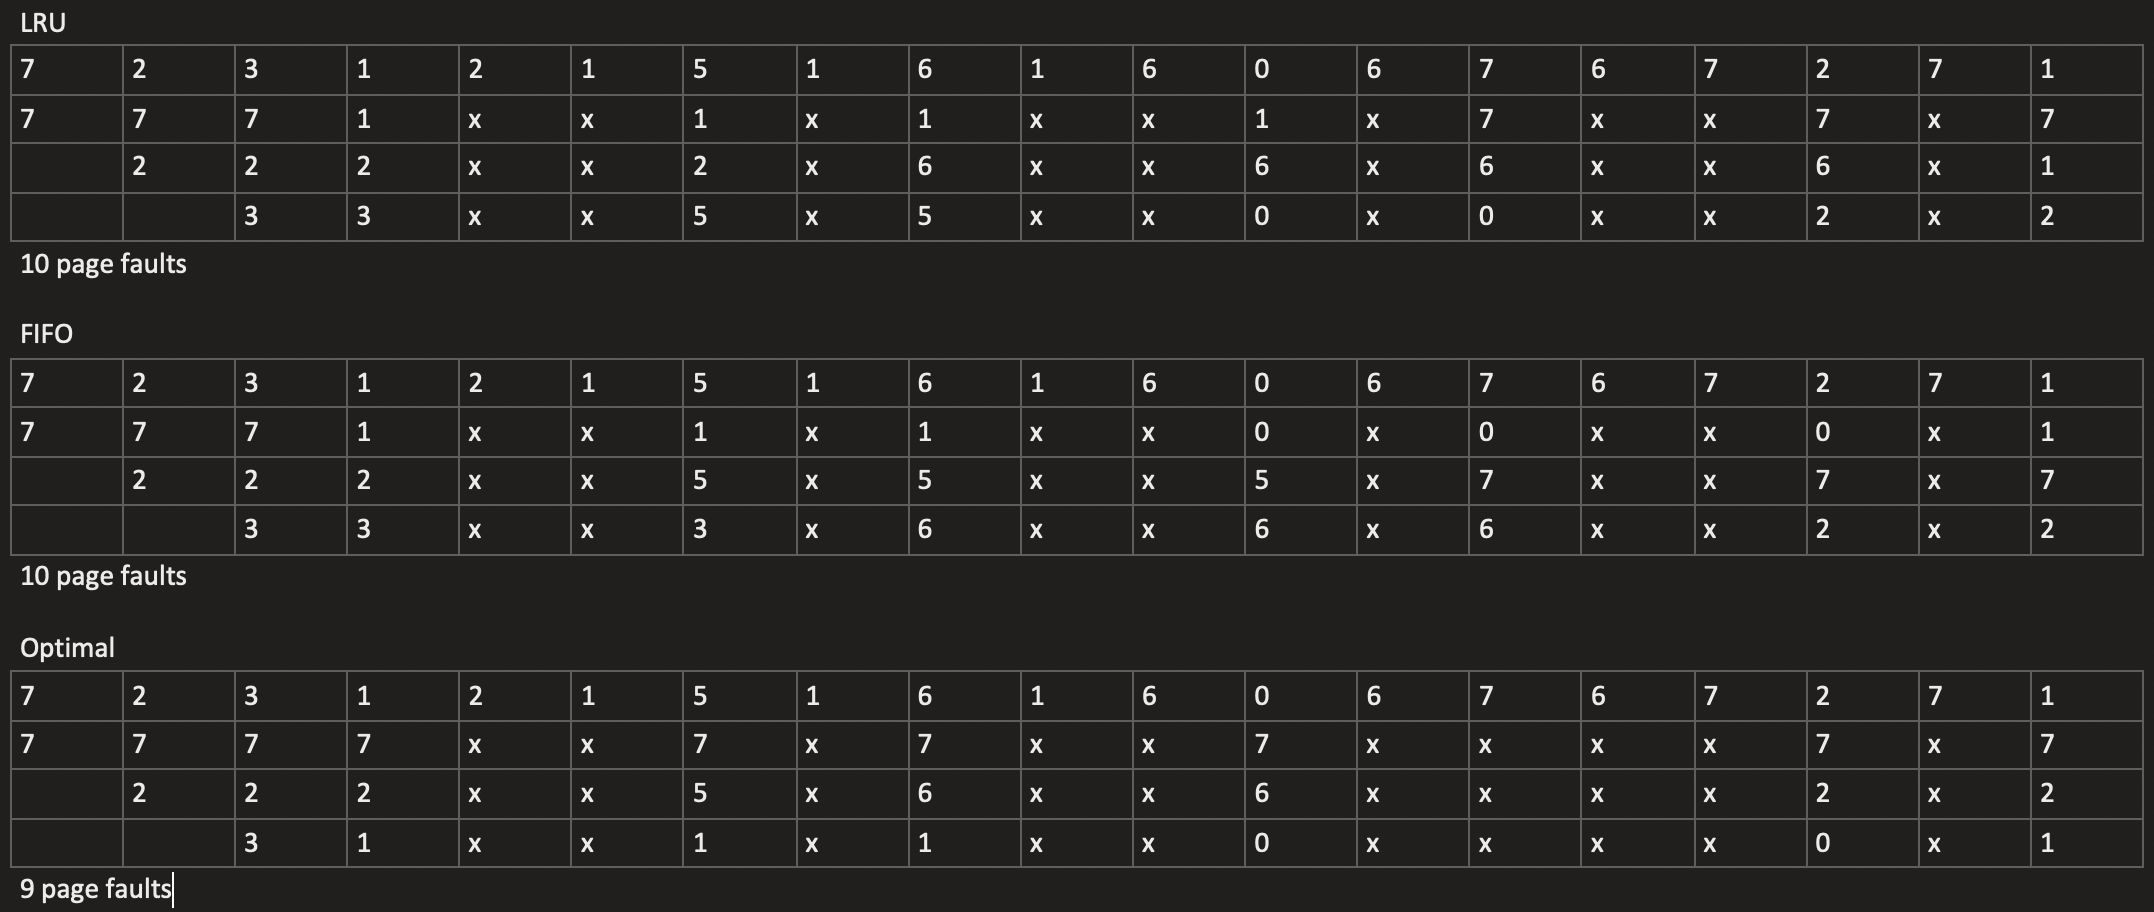
\includegraphics[scale=0.4]{COMS352HW8Q3}\\
\section*{Question 4}
Thrashing occurs when a process does not have the minimum number 
of pages allocated resulting in it to continuously page fault. The 
system detects thrashing by  comparing the CPU utilization to 
the degree of multiprogramming and determines if the CPU 
utilization is too high compared to the multiprogramming. To 
Stop thrashing we need to decrease the degree of multiprogramming
taking place.
\section*{Question 5}
If $\Delta$ is a very small value, then the processes pages are 
not all in memory and will get scheduled because all pages are 
in the working set. The number of page faults will increase. If 
$\Delta$ is a very large value, then the process doesn't have enough pages
and prevents the process from getting scheduled. This will result 
in an incease in page faults.s
\end{document}